\documentclass[a4paper,11pt]{article}
\usepackage[T1]{fontenc}
\usepackage[dvipsnames]{xcolor} % for setting colors
\usepackage{pgfgantt}
\usepackage[utf8]{inputenc}
\usepackage{graphicx}

\usepackage{mathtools}
%\renewcommand\familydefault{\sfdefault}
%\usepackage{tgheros}
\usepackage{xcolor}
\usepackage{amsmath,amssymb,amsthm,textcomp}
\usepackage{enumerate}
\usepackage{multicol}
\usepackage[ruled,vlined]{algorithm2e}
\usepackage{listings}
\newtheorem{theorem}{Lemma}
\usepackage{subfig}
\usepackage{float}
\usepackage{ifthen}
\usetikzlibrary{matrix,calc}
\usepackage{pgf,tikz,pgfplots}
\usepackage{minted}
\usepackage[T1]{fontenc}
\usepackage{textcomp}
\usepackage[scaled]{beramono}

\usepackage{mathrsfs}
\usepackage{mathtools}
\usepackage{natbib}
\DeclarePairedDelimiter\ceil{\lceil}{\rceil}
\DeclarePairedDelimiter\floor{\lfloor}{\rfloor}

\usepackage{chngcntr}
\counterwithin*{equation}{section}
\counterwithin*{equation}{subsection}

\usepackage{amsmath}
\addtolength{\topmargin}{-60pt}
\addtolength{\textheight}{120pt}
\newcommand{\sfunction}[1]{\textsf{\textsc{#1}}}

\usepackage{geometry}
\geometry{left=25mm,right=25mm,%
	bindingoffset=0mm, top=20mm,bottom=20mm}
\usepackage{indentfirst}

\linespread{1.3}
\usepackage{amsmath,amssymb,graphicx, float}
\usepackage{booktabs}
\usepackage{hyperref}
\hypersetup{
    colorlinks=true,
    linkcolor=blue,
    urlcolor=blue,
}
\newcommand{\cf}[1]{{\small \textt{#1}}}
\newcommand{\linia}{\rule{\linewidth}{0.5pt}}

% custom theorems if needed
\newtheoremstyle{mytheor}
    {1ex}{1ex}{\normalfont}{0pt}{\scshape}{.}{1ex}
    {{\thmname{#1 }}{\thmnumber{#2}}{\thmnote{ (#3)}}} 

\theoremstyle{mytheor}
\newtheorem{defi}{Definition}

% my own titles

\makeatletter
\renewcommand{\maketitle}{
	\begin{center}
		\vspace{2ex}
		{\huge \textsc{\@title}}
		\vspace{1ex}
		\\
		\linia\\
		\@author \hfill \@date
		\vspace{4ex}
		
	\end{center}
}
\makeatother
%%%custom secton title
\usepackage{titlesec}
% \titleformat{\section}[block]{\LARGE \scshape \bfseries\filcenter}{}{1em}{}
% \titleformat{\subsection}[hang]{\Large \scshape \bfseries}{}{1em}{}
% \titleformat{\subsubsection}[hang]{\scshape \bfseries}{}{1em}{}
% custom footers and headers
\usepackage{fancyhdr}
\pagestyle{fancy}
\lhead{}
\chead{}
\rhead{}
\lfoot{}
\cfoot{Page \thepage}
\rfoot{}
\renewcommand{\headrulewidth}{0pt}
\renewcommand{\footrulewidth}{0.4pt}
%
\usepackage{booktabs}
\newcommand{\bigcell}[2]{\begin{tabular}{@{}#1@{}}#2\end{tabular}}
% code listing settings
\pgfplotsset{compat=1.5, width=15cm, height=10cm, scale only axis}
\usepackage{listings}
\lstset{
	language=Python,
	basicstyle=\ttfamily\small,
	aboveskip={1.0\baselineskip},
	belowskip={1.0\baselineskip},
	columns=fixed,
	extendedchars=true,
  breaklines=true,
  tabsize=4,
  prebreak=\raisebox{0ex}[0ex][0ex]{\ensuremath{\hookleftarrow}},
	frame=lines,
	showtabs=false,
	showspaces=false,
	showstringspaces=false,
	keywordstyle=\color[rgb]{0.627,0.126,0.941},
	commentstyle=\color[rgb]{0.133,0.545,0.133},
	stringstyle=\color[rgb]{01,0,0},
	numbers=left,
	numberstyle=\small,
	stepnumber=1,
	numbersep=10pt,
	captionpos=t,
	escapeinside={\%*}{*)}
}
\usepackage{subfiles}
%%%----------%%%----------%%%----------%%%----------%%%

\title{CS2800 Algorithms Assignment \textnumero{} 4}


\date{17/02/2020}

\begin{document}
\begin{titlepage}
	\centering
	
\includegraphics[width=0.15\textwidth]{ IIT.png} \par\vspace{1cm}
	{\scshape\LARGE Indian Institute of Technology, Madras \par}
	\vspace{0.5cm}
	{\scshape\large Department of Computer Science \& Engineering \par}
	\vspace{0.5cm}
	{\scshape\large Undergraduate Research in Computer Science - I\par}
	\vspace{1.5cm}
	{\scshape\Large Project Report\par}
	\vspace{1.5cm}
	{\scshape\Large A Probabilistic Programming Library\\ using Effect Handlers in Multicore OCaml \par}
	\vspace{1.5cm}
	{\huge\bfseries  \par}
	\vspace{2cm}
	{\Large\itshape 
	Arnhav Datar - \href{mailto:cs18b003@smail.iitm.ac.in}{cs18b003@smail.iitm.ac.in} \\ 
	under Dr. KC Sivaramakrishnan\par}
	\vfill

% Bottom of the page
	{\large \today\par}
\end{titlepage}

\tableofcontents



% \lstlistoflistings

\section{Acknowledgements}
\noindent
This work has been done primarily because of the guidance of Dr. KC Sivaramakrishnan and Dr. Tom Kelly. I would like to thank them both for their constant support and valuable suggestions. I would also like to thank Dr. Yadu Vasudev for his coordination of the UGRC course. 

\section{Abstract}

In this report, we present EffPPL, a shallowly embedded domain-specific probabilistic programming library in Multicore OCaml made using effect handlers. EffPPL has the capability to perform approximate Bayesian inference for models using continuous random variables. EffPPL uses the Hamiltonian Monte Carlo for performing the inference. We briefly explain the implementation of the same. In this report we also explore potential applications of EffPPL. Furthermore, we compare EffPPL's performance against Stan~\cite{stan}(one of the most highly optimised probabilistic programming languages)  for a linear regression model, to show the practicality of EffPPL. 

\section{Introduction}

\subsection{Probabilistic Programming}

Bayesian modelling lies at the heart of Machine Learning. Bayesian modelling involves assigning the parameters of the model some prior distributions, followed by giving a set of conditions, wherein, we compute the likelihood that the parameters could generate the observed data. This is then used to generate the posterior distribution. 

Since exact Bayesian inference is often intractable, we work towards approximate Bayesian inference. Probabilistic programming languages(PPLs) have been used for performing approximate Bayesian inference ~\cite{Baydin_2019} in complex generative models. PPLs allow us to create these models using simpler models and probability distributions. Probabilistic Programming ~\cite{vandemeent2018introduction} involves the construction of inference problems and the development of corresponding evaluators, that computationally characterize the denoted conditional distribution.

Probabilistic programming has shown applications ~\cite{appl} in the fields of computer vision, cryptography, quantitative finance, biology and reliability analysis. Until recently, probabilistic programming was limited in scope, and most inference algorithms had to be written manually for each task. Recently with availability of greater compute capability, larger datasets and advances in concurrent and parallel programming, the probabilistic programming paradigm is becoming ubiquitous. 

\subsection{Effect Handlers}

Effect handlers~\cite{effects} are a mechanism for modular programming with user-defined effects. Similar to defining new exception values, the user can define their own effects. These are handled with an effect handler. But unlike exceptions, effect handlers permit the control to go back to where the effect was performed, but also save the context necessary for going back in a data structure. This ability to suspend and resume computations later allows new programming paradigms, including algorithmic differentiation and probabilistic programming. Multicore OCaml incorporates effect handlers as a way of supporting concurrency primitives. The example below illustrates effect handlers:

\begin{listing}[H]
\centering
\begin{minted}[linenos, frame=lines,tabsize=2]{ocaml}
let comp () =
     print_string "0 ";
     print_string (perform E);
     print_string "3 "

let main () =
     try
        comp ()
     with effect E k ->
         print_string "1 ";
         continue k "2 ";
         print_string "4 "
\end{minted}

\caption{Demonstrating Effect Handlers in Multicore OCaml}
\end{listing}
\vspace{0.5cm}
\hrule
\vspace{0.5cm}
\textbf{Output} : 0 1 2 3 4 
\vspace{0.5cm}
\hrule
\vspace{0.5cm}
% 
\noindent
\textbf{Control Flow of the above program}
\begin{enumerate}
    \item Function \lstinline{comp()} is tried
    \item Going sequentially it prints 0.
    \item Upon seeing the \lstinline{(perform E)}, suspends the current computation and reifies it as a delimited continuation~\cite{delim}.
    \item Going sequentially it prints 1.
    \item Here upon seeing the delimited continuation it returns 2 back to \lstinline{comp()}, wherein it prints 2.
    \item Continuing \lstinline{comp()} it prints 3.
    \item Then, it finally continues the remaining part of the effect E. This is similar to returning from a function. It prints 4.
\end{enumerate}

 For further examples of effect handlers in Multicore OCaml refer to the \texttt{effects-examples}~\cite{ocaml-multicore} repository on GitHub. Effect handlers have been used for probabilistic programming languages~\cite{hack,pyro}. Effect handlers are a great fit for probabilistic programming since they can be used to implement algorithmic differentiation, and the non-local control flow necessary for expressing probabilistic programming constructs. 


% \section*{Hypothesis}



\section{Related Work}


There have been many probabilistic programming efforts both as libraries and as independent languages. The development of these languages has sped up in the past few years, there being a lot of languages/libraries developed in the last 5 years. Some noteworthy mentions are Stan~\cite{stan}, Pyro~\cite{pyro}, HackPPL~\cite{hack}, CuPPL~\cite{collins2020probabilistic}, OwlPPL~\cite{roy2020probabilistic} and LF-PPL~\cite{zhou2019lfppl}. 

There have been a number of prior works that implement PPLs in OCaml. IBAL ~\cite{IBAL} and Hansei ~\cite{Hansei} are PPLs that have been implemented in OCaml. However, the languages are not universal languages. Universal probabilistic languages can have an unlimited number of random variables. By contrast EffPPL can handle an unlimited number of random variables. Furthermore, they are not implemented using effect handlers as opposed to the EffPPL. They also tend to use simpler inference algorithms as compared to the Hamiltonian Monte Carlo. Also these are programming languages and thus they can only serve the purpose of probabilistic programming. EffPPL being a shallowly embedded~\cite{dsl} DSL in OCaml can use all the other capabilities of OCaml.

Kiselyov et al.~\cite{Kiselyov2009Embedded} present an embedded probabilistic programming library in OCaml. This library is one of the first works of an embedded PPL in OCaml. However, it used simple inference algorithms like the exact inference for discrete distributions and the importance sampling for continuous distributions. EffPPL on the other hand uses the Hamiltonian Monte Carlo. The library also does not use effect handlers as compared to EffPPL. 

Recently, Anik Roy developed OwlPPL~\cite{roy2020probabilistic}, a universal embedded PPL using the Owl library~\cite{wang2018owl}, a general-purpose numerical library for OCaml. However, similar to its predecessors, it does not use effect handlers. It implements a variety of inference algorithms ranging from simple enumeration to MCMC methods like Metropolis-Hastings. It does not implement more modern inference algorithms like the Hamiltonian Monte Carlo(HMC)~\cite{betancourt2018conceptual}, Stochastic gradient Hamiltonian Monte Carlo(SGHMC)~\cite{sghmc} and the No U-Turn Sampler(NUTS)~\cite{hoffman2011nouturn}. EffPPL on the other hand implements the HMC.  

 Effect handlers have been used for developing modern universal PPLs like HackPPL~\cite{hack} from Facebook and Pyro~\cite{pyro} from Uber. Pyro is built on Poutine which is a library of effect handlers. Edward~\cite{tran2017deep} is a modern probabilistic modelling library that supports concurrency, but it does not use effect handlers and is not universal. Given the successes of these languages, EffPPL is our attempt at taking advantage of effect handlers in Multicore OCaml to implement an universal PPL. Table \ref{ppls} is a detailed table summarising the probabilistic programming languages referred to in this report.

\begin{table}[H]
	\centering
    \caption{A collection of PPLs}
	\begin{tabular}{|c|c|c|}
		\toprule
		PPL & Host Language & Reference \\	
		\midrule
		\midrule
		BUGS        & N/A               & ~\cite{gilks1994language} \\
		IBAL        & OCaml             &  ~\cite{IBAL} \\
		JAGS        & N/A               &  ~\cite{jags} \\
		Church      & LISP              &  ~\cite{goodman2012church} \\
		HANSEI      & OCaml             &  ~\cite{Hansei}\\
		Infer.NET   & F\#               &  ~\cite{wang2011using} \\
		Anglican    & Clojure           &  ~\cite{tolpin2016design} \\
%		WebPPL      & JavaScript (node) &  ~\cite{  \\
		Pyro        & Python            & ~\cite{pyro}  \\
		OwlPPL      & OCaml             &  ~\cite{roy2020probabilistic} \\
		Edward  	& Python            &   ~\cite{tran2017deep}\\
		Stan    	& C++,Python,R      &  ~\cite{stan}\\
%		PyMC        & Python            &  \\
		HackPPL		& Hack				& ~\cite{hack} \\
		CuPPL       & CUDA 				& ~\cite{collins2020probabilistic} \\
		LF-PPL 		& Python 			& ~\cite{zhou2019lfppl} \\
		\bottomrule
	\end{tabular}
	\label{ppls}
\end{table}


\section{Implementation}
    
    \subsection{Language Design}
    
    For the user to have an intuitive and easily understandable interface to create the models the language tries to mirror OCaml with the only difference being using \lstinline{let*} as opposed to \lstinline{let}. The applications described in section \ref{sec:app} show how useful this design style is. A simple example illustrating the same is given below:
    
    \begin{listing}[H]\centering
    \begin{minted}[linenos, frame=lines,tabsize=2]{ocaml}
    let sum_of_normals () = 
    	let* x1 = normal 0. 1. in
    	let* x2 = normal 0. 1. in
    	x1 +. x2
    
    \end{minted}
    
    \caption{Sum of standard normal variables}
    \end{listing}
    % \begin{listing}[H]\centering
    % \begin{minted}[linenos, frame=lines,tabsize=2]{ocaml}
    % let sum_of_floats () = 
    % 	let x1 = 2. in
    % 	let x2 = 3. in
    % 	x1 +. x2
    
    % \end{minted}
    
    % \caption{Sum of standard normal variables}
    % \end{listing}
    
    
    The language has been implemented as a shallowly embedded~\cite{dsl} DSL in OCaml. Being a DSL, other constructs of OCaml such as the let, if, for statements along with functions written in OCaml can be used within the library functions.
    
    OCaml post version 4.08 allowed the defining of a custom \lstinline{let*} binding. So in order to create a shallowly embedded DSL we redefine a few primitives such as the \lstinline{let*} and arithmetic operators(such as \lstinline{+.}, \lstinline{-.}, \lstinline{*.}). We also add functions(such as \lstinline{normal}) to simulate primitive distributions and observe random variables.
    
    The newly defined functions/operators invoke effect handlers upon being called. We take advantage of effect handlers ability to simulate user defined effects to overload the meaning of arithmetic operators suitably for the models. This ensures that the domain-experts of probabilistic programming need not be familiar with effect handlers to use the library to its fullest potential.
    
    
    \subsection{The Hamiltonian Monte Carlo}

    The Hamiltonian Monte Carlo(HMC) has proven a remarkable empirical success in the recent years~\cite{betancourt2018conceptual}. Its variant the No-U-Turn Sampler is the industry standard and is used by a lot of recent PPLs~\cite{stan,pyro,tran2017deep}. The Hamiltonian Monte Carlo algorithm~\cite{hoffman2011nouturn} used in EffPPL is described below: \\
    
	\begin{algorithm}[H]
		\SetAlgoLined
		Given $\theta^0, L, \epsilon, \mathcal{L}, M$:\\
		\For{$m = 1~ to~ M$}{
		    Sample $r^0 \sim \mathcal{N}(0, I)$\\
		    $\theta^m \gets \theta^{m-1} $\\
		    $\theta' \gets \theta^{m-1} $\\
		    $r' \gets r^{0} $\\
			\For{$i = 1~ to~ L$} {
			    $(\theta', r') \gets Leapfrog(\theta', r', \epsilon)$\\
			}
			With probability $\min \{1, \frac{\exp\left(\mathcal{L}(\theta') - 0.5 \cdot r' \cdot r' \right)}{\exp\left(\mathcal{L}(\theta^{m-1}) - 0.5 \cdot r^0 \cdot r^0\right)} \}$ set $\theta^m \gets \theta' $ and $r^m \gets -r' $\\
		}
		\textbf{function} $Leapfrog(\theta', r', \epsilon):$\\
		    $~~~~r' \gets r' + (\epsilon / 2) \nabla_\theta \mathcal{L}(\theta)$\\
		    $~~~~\theta' \gets \theta' +  (\epsilon ) r'$\\
	        $~~~~r' \gets r' + (\epsilon / 2) \nabla_\theta \mathcal{L}(\theta')$\\
		return $(\theta', r')$
		\caption{Hamiltonian Monte Carlo}
	\end{algorithm}
	\vspace{0.5cm}
	We briefly elaborate the various components of the HMC:
	\begin{enumerate}
	    \item \textbf{Generating Transitions:}\\
    	Starting from the current value of the parameters $\theta^0$, a transition is made in two steps
    	\begin{enumerate}
    	    \item A value for the momentum is drawn from standard normal variables in the step $r^0 \sim \mathcal{N}(0, I)$. 
    	    \item Now the joint system of $(\theta, r)$ is solved using the Hamiltonian equations
    	    \begin{align*}
    	        \frac{d\theta}{dt} &= \frac{dH}{dr}\\
    	        \frac{dr}{dt} &= - \frac{dH}{d\theta}
    	    \end{align*}
    	\end{enumerate}
    	Betancourt et. al.~\cite{betancourt2018conceptual} explains the mathematics behind the equations. For further details kindly refer the same. 
    	\item \textbf{Leapfrog Integrator:}\\
    		The last part leaves a two-state differential equation to solve. EffPPL uses the leapfrog integrator, which is a numerical integration algorithm. We use it as a function above which is repeated $L$ times. This is the equivalent of the passing $L\epsilon$ time in a physical system. 
		\item \textbf{Metropolis Accept Step:}\\ If the Leapfrog integrator was a perfect integrator this step would have been unnecessary.  To account for numerical errors during integration a Metropolis acceptance step is applied at the end of the algorithm. 
	\end{enumerate}
	
	As can be seen, we need to compute $\nabla_\theta \mathcal{L}$ twice in a leapfrog iteration. We can therefore conclude that we need to calculate gradients at least $2ML$ times. This value may get larger for higher precision tasks. Since it is a heavily repeated complex part of the algorithm, it is necessary to make it efficient. To achieve the same we use effect handlers as described below. 
	 
	\subsection{Algorithmic Differentiation}
    
    The Hamiltonian Monte Carlo requires the algorithmic differentiation~\cite{adml} to compute the updates that are need to be performed.  We use the method described in Margossian et. al.~\cite{Margossian_2019}. We use the reverse mode differentiation~\cite{reverse} since its more suited when there are more parameters as compared to return values.
    
    The traditional way of implementing reverse-mode AD is to rely on a tape or a computation graph or an explicit data structure. Wang et al.~\cite{wang2019demystifying} shows how to use delimited continuations to implement reverse mode AD using delimited continuations to inject backward computation as a part of the normal program control flow. While Wang et al use operator overloading from Scala, we achieve the same effect in OCaml by using effect handlers. Given below we have given the cases for addition and multiplication for calculating the gradients.
    
\begin{listing}[H]\centering
\begin{minted}[linenos, frame=lines,tabsize=2]{ocaml}
| r -> 
	r.d <- 1.0; 
	ls := modif_der !ls r.v r.d;
	(r)
| effect (Add(a,b)) k ->
	let t = {v = a.v +. b.v; d = 0.; m=1.} in
	ignore (continue k t);
	a.d <- a.d +. t.d;
	b.d <- b.d +. t.d; 
	ls := modif_der !ls a.v a.d;
	ls := modif_der !ls b.v b.d;
	(x)
	
| effect (Mult(a,b)) k ->
	let t = {v = a.v *. b.v; d = 0.;  m=1.} in
	ignore (continue k t);
	a.d <- a.d +. (b.v *. t.d);
	b.d <- b.d +. (a.v *. t.d);
	ls := modif_der !ls a.v a.d;
	ls := modif_der !ls b.v b.d;
	(x)
\end{minted}
  
\caption{Algorithmic Differentiation}
\end{listing}   
    As we can see, we initially compute the values from the addition and multiplication of \lstinline{a} and \lstinline{b} in \lstinline{t.v}, and then use delimited continuation to send the value for further computation.  To illustrate how this works we show an example for $z = 2x + xy$ for $x=1$ and $y=2$. By simple calculus we can see that
    \begin{align}
        \partial z / \partial x &= 2 + y = 4\\
        \partial z / \partial y &= x ~~= 1
    \end{align}
    
    
    
    In EffPPL, \lstinline{z} can be expressed as \lstinline{Add(Mult(2,x), Mult(x,y))}. The control flow is as follows:
    \begin{enumerate}
        \item Initially \lstinline{Mult(2,x)} is evaluated, here simply \lstinline{x.v} is computed as $2$ and sent to the continuation. Let this term be called \lstinline{z1}.
        \item Similarly, \lstinline{Mult(x,y)} is evaluated here too \lstinline{x.v} is computed as $4$ and sent to the continuation. Let this term be called \lstinline{z2}.
        \item Then the addition is computed as $6$ and sent to the continuation.
        \item Finally we reach \lstinline{r}, wherein we store the derivative of $z$ with respect to itself as 1 in \lstinline{ls}.
        \item Now we return to \lstinline{Add(z1, z2)}. Here since \lstinline{t.d} has been updated to 1 both the derivatives of \lstinline{z} with respect to \lstinline{z1} and \lstinline{z2} get the value 1.0
        \item The program then goes to \lstinline{Mult(x,y)}. Here \lstinline{t.d} is 1 and \lstinline{a.v = 1} while \lstinline{b.v}=2, this makes \lstinline{a.d}(x) as 2 and \lstinline{b.d}(y) as 1. Hence, at this point the derivatives stored in ls are:
        \begin{enumerate}
            \item $\partial z / \partial x = 2.0$
            \item $\partial z / \partial y = 1.0$
            \item $\partial z / \partial z = 1.0$
        \end{enumerate}
        \item Finally the program sees \lstinline{Mult(2,x)}. Again \lstinline{t.d} is 1 therefore \lstinline{a.d}(2) gets updated to 1 and \lstinline{b.d}(x) gets updated to $2+2 = 4$. But the \lstinline{modif_der} recognises 2 to be a constant and does not consider it. So finally we get the derivatives as :
        \begin{enumerate}
            \item $\partial z / \partial x = 4.0$
            \item $\partial z / \partial y = 1.0$
            \item $\partial z / \partial z = 1.0$
        \end{enumerate}
    \end{enumerate}
    
    Therefore, we finally get the derivative of z with respect to x as 4, while we get the derivative of z with respect to y as 1 as was computed in equations (1) and (2). 
    
    \subsection{Testing}
    
    \subsubsection{Algorithmic Differentiation}
        To test the algorithmic differentiation we used two methods
        \begin{enumerate}
            \item\textbf{Hand calculation of gradients:} this was done for a few models by writing a script and checking if the values actually give the expected gradients
            \item\textbf{Plots:} Figures \ref{test1} and \ref{test2} represent the plots for the gradients of sum of normal variables and the product of normal variables. As can be seen the sum of normal variables closely mirrors a normal slope, while the product of normal variables is a normal variable multiplied with the gradient of a normal variable.
        \end{enumerate}
        We tried these two tests because at times the the gradient for simple models was easily calculable so we checked manually by calculating gradients. But such tests did not guarantee that the sampling was being done randomly neither did they ensure the same for all values. Plots help us visualise the same.   
    
    \begin{figure}[H]
    \centering
    \begin{minipage}{0.49\textwidth}
        \centering
        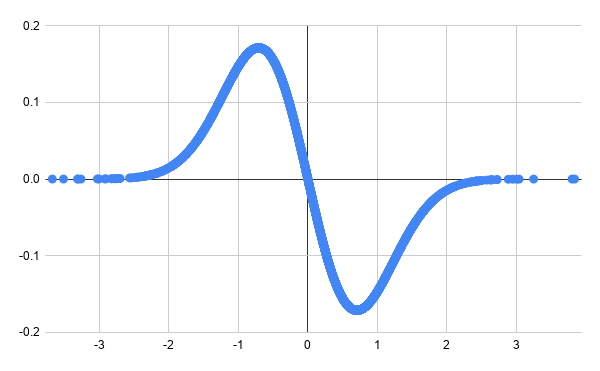
\includegraphics[width=0.99\textwidth]{testing/diff.png} % first figure itself
        \caption{Sum of normals}
        \label{test1}
    \end{minipage}\hfill
    \begin{minipage}{0.49\textwidth}
        \centering
        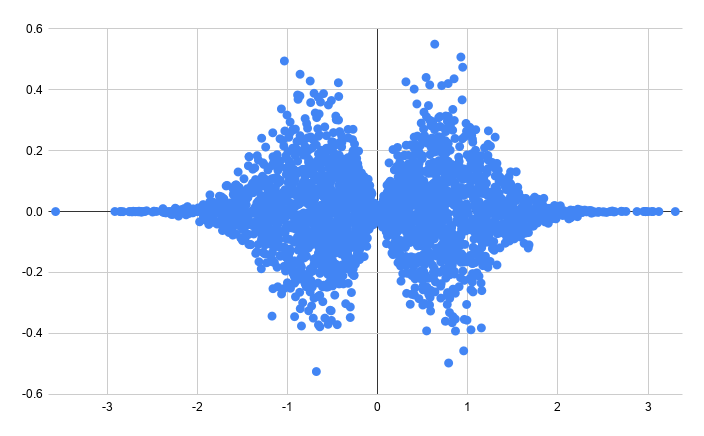
\includegraphics[width=0.99\textwidth]{testing/diff1.png} % second figure itself
        \caption{Product of normals}
        \label{test2}
    \end{minipage}
    
    \end{figure}
        
        
    \subsubsection{Samplings}
    
        To check the final HMC was functioning correctly we sampled from a variety of distributions and checked if their means, medians and standard deviations match with the expected values. This was done for all standard distributions along with some distributions involving combinations of standard distributions. One exception is Cauchy distribution whose mean and variance is undefined. We also plotted the same and checked if the plots match the expected distributions as can be seen in section \ref{vardist}.
        
        We also perform the Kolmogorov-Smirnov test~\cite{kstest} (K-S test) on these samples, to find low values implying that the sampling is accurate. The Kolmogorov-Smirnov test is a non-parametric goodness-of-fit test, and is used to determine whether an underlying probability distribution differs from a hypothesized distribution. Figure \ref{fig:kst} illustrates how the statistic of the K-S test is calculated.
        \begin{figure}[H]
            \centering
            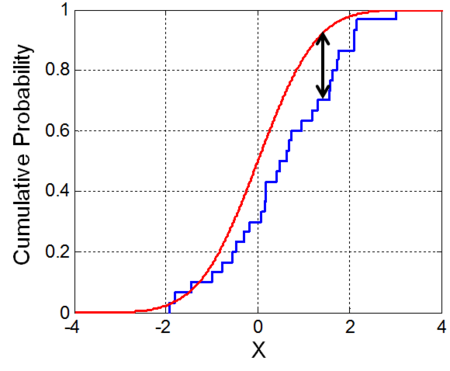
\includegraphics{ks.png}
            \caption{The red line is a model CDF, the blue line is an empirical CDF, and the black arrow is the K–S statistic.}
            \label{fig:kst}
        \end{figure}
        sl
        As can be seen from the figure above when the K-S statistic is low(close to 0), it implies that the sampling is good representation of the proposed distribution. The detailed table (Table \ref{kstests}) showing the values of all K-S tests along with the number of samples drawn for each can be found below. 
        

\begin{table}[H]
	\centering
    \caption{K-S Test results}
	\begin{tabular}{|c|c|c|}
		\toprule
		Distribution   & {Samples} & {K-S test statistic} \\
		\midrule
		\midrule
	
        Sum of normals & 10000                       & 0.02704                               \\
        Chi-squared    & 2000                        & 0.05836                               \\
        exponential    & 10000                       & 0.08071                               \\
        $Beta(1,1)$      & 10000                       & 0.00972                               \\
        $Beta(1,2)$     & 5000                        & 0.01866                               \\
        $Beta(2,1)$      & 5000                        & 0.02334                               \\
        Continous      & 5000                        & 0.00645            \\          
		\bottomrule
	\end{tabular}
	\label{kstests}
\end{table}
    
\section{Applications}
    \label{sec:app}
    In this section, we describe a few application that have been implemented using EffPPL. As can be seen with the accompanying code, the models are quite naturally expressed in EffPPL. We have provided a detailed list of functions and primitives used in EffPPL in Table \ref{key} in the Appendix. 
    % 
    \subsection{Machine Learning models}
        Probabilistic programming libraries have shown many applications in the domains of machine learning and deep learning. We present two simple and fundamentals applications here.
        \subsubsection{Linear Regression}
            The 1-D linear regression model is the following, with a single predictor and a slope and intercept coefficient, and normally distributed noise. This model can be written using standard regression notation as
            \begin{equation*}
                Y_n \sim \mathcal{N}( \alpha + \beta X_n , \sigma )
            \end{equation*}
            The code for performing inference here is given below:\\
\begin{listing}[H]\centering
\begin{minted}[linenos, frame=lines,tabsize=2]{ocaml}
let lin obs_points ax ay () =
	let* m = normal 2. 3. in 
	let* c = normal 0. 10. in 
	let* s = exp 5. in 
	for i = 0 to (obs_points-1) do 
		observe (mk ay.(i) -. m*.mk ax.(i) -. c) 
		(logpdf Primitive.(normal 0. (get s)))
	done ;
	m 
\end{minted}
\caption{Linear Regression in EffPPL}
\end{listing}
    A walkthrough through the same is as follows:
    \begin{enumerate}
        \item We initially pass \lstinline{obs_points, ax, ay} as parameters to \lstinline{lin}.
        \item Here we give some prior that we may have about \lstinline{m,c,s}. As can be seen the priors given by us are not particularly accurate for the expected values of $m=3, c=2$ and $s = 1$. If the user is very unsure, he can simply choose the prior as a normal distribution with a large standard deviation.
        \item We then use a for loop to iterate over all the observation points. In the statement\\ \lstinline{observe (mk ay.(i) -. m*.mk ax.(i) -. c)   (logpdf Primitive.(normal 0. (get s)))}\\ we try to say that $(y(i) - m*x(i) - c) \sim \mathcal{N}(0, s)$. The first term in the code statement denotes the L.H.S. while the next statement denotes a function that takes in an input float and return the logpdf of a normal distribution. 
    \end{enumerate}
    We use the logpdf, because we need to compute the product of all pdfs in the HMC implementation. Most hardwares won't be able to deal with floating point numbers this small, hence we convert it to log and and add it up in the HMC implementation.  To test the correctness we gave it data which was sampled from $\mathcal{N}( 3x + 2 , 1 )$. When we did an HMC sampling we got the mean slope as $3.02$ and the constant as $1.84$. A similar value was obtained via Stan. More details on the same can be found in section \ref{sec:eval}. 


\begin{figure}[H]
    \centering
    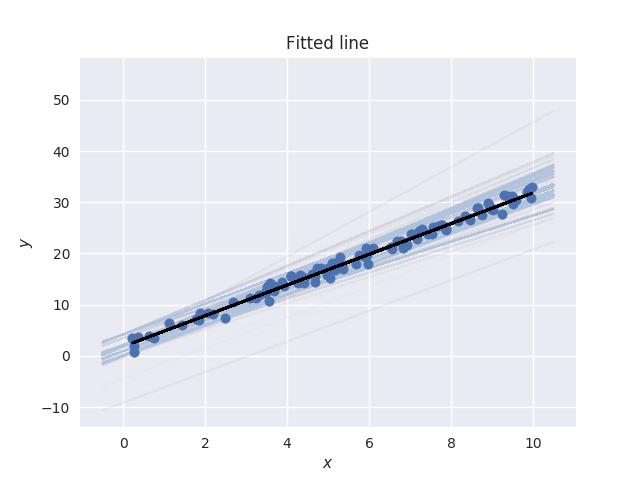
\includegraphics[width=8cm]{machine_learning/linreg.png}
    \caption{Linear Regression Plot}
    \label{fig:linref}
\end{figure}
   Figure \ref{fig:linref} is a plot showing sampled lines and the mean line. The black line indicates the line with the mean slope and constant. While the other faint blue lines indicate samples that PPL drew. 
    
    
        \subsubsection{Binary Classification}
        
        The task of classification is one of the most famous ones in machine learning. The fundamental task revolves around classifying the elements of a set into two groups on the basis of previous data. Many algorithms(such as support vector machines, random forests etc.) have been used to tackle the problem. In a PPL setting we propose an elementary algorithm for classification. The idea behind it is that for an ideal linear a correctly classified point should be much more likelier than an incorrectly classified point. This can be seen in the code below as we give a logpdf of +1 when we correctly classify and -1 when we incorrectly classify. The function which does so is:\\ \lstinline{(fun x -> if((Float.mul x ay.(i)) > 0.) then 1.0 else -1.0)}.\\
        The function basically checks if the predicted and real $y$ have the same sign, if yes it returns 1 else -1 as the logpdf. 
        
\begin{listing}[H]\centering
\begin{minted}[linenos, frame=lines,tabsize=2]{ocaml}
let class obs_points ax1 ax2 ay () =
  let* m1 = normal 0. 2. in 
  let* m2 = normal 0. 2. in 
  for i = 0 to (obs_points-1) do 
    observe (m1*.mk ax1.(i) +. m2*.mk ax2.(i) +. mk 1.0) 
	(fun x -> if( (Float.mul x ay.(i)) > 0.) then 1.0 else -1.0)
  done;
  m1
\end{minted}
\caption{Classification in EffPPL}
\end{listing}        
        % \subsubsection{Neural Network}
        
        Given below in figure \ref{fig:class} are some of the classifications we have sampled, with the central black line representing the mean of the parameters. 
        \begin{figure}[H]
            \centering
            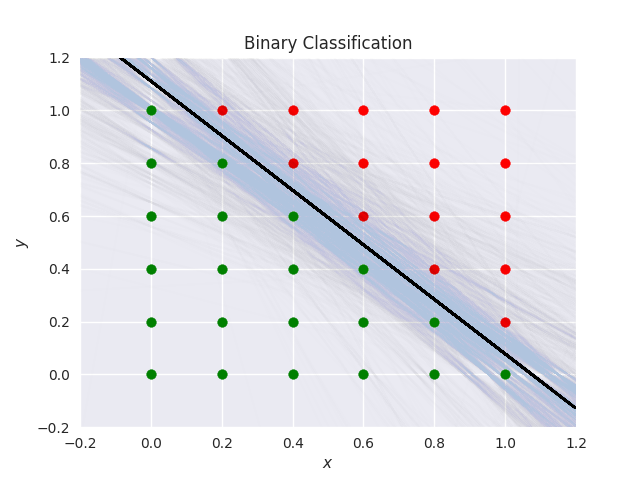
\includegraphics[width=7cm]{machine_learning/class.png}
            \caption{Classification Plot}
            \label{fig:class}
        \end{figure}
        
    \subsection{Time Series Models}
    In mathematics, a time series is a series of data points indexed (or listed or graphed) in time order. Time series analysis comprises methods for analyzing time series data in order to extract meaningful parameters of the data. In this section we list one common example of time series analysis
        \subsubsection{Auto-Regressive Model}
         The auto-regressive model specifies that the output variable depends linearly on its own previous values and on a stochastic term(usually a normal variable). Here we consider the simplest case(AR(1)) wherein the output is only dependant on its last value. Figure \ref{fig:ar} is a plot for an AR(1) model for $\alpha = 5$ and $\beta = 0.4$:
         \begin{figure}[H]
             \centering
             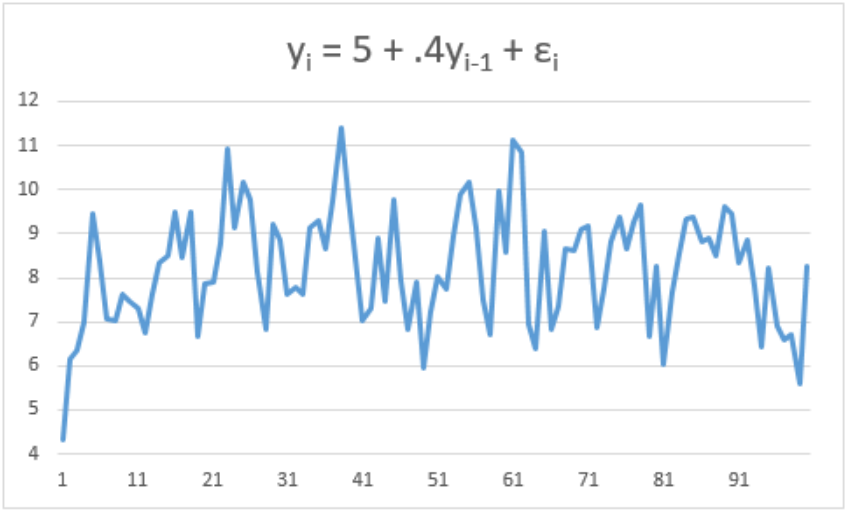
\includegraphics[width = 8cm]{time-series/ar_plot.png}
             \caption{AR(1) model}
             \label{fig:ar}
         \end{figure}
        The auto-regressive model can therefore be defined as follows:
        \begin{equation*}
            Y_n \sim \mathcal{N}( \alpha + \beta Y_{n-1} , \sigma )
        \end{equation*}
        where $\{Y_i\}$ is a sequence of random variables taken from a time-series. The equivalent EffPPL code to infer the parameters $\alpha$ and $\beta$ can be found below.
        
\begin{listing}[H]\centering
\begin{minted}[linenos, frame=lines,tabsize=2]{ocaml}
let autoreg obs_points ay () =
  let* alp = normal 1. 1. in 
  let* bet = normal 1. 1. in 
  let* s = exp 5. in 
	
  for i = 0 to (obs_points-2) do 
    observe ((mk ay.(i+1)) -. alp -. bet*.(mk ay.(i))) 
    (logpdf Primitive.(normal 0. s))
  done
\end{minted}
\caption{Auto-Regressive model in EffPPL}
\end{listing}      

    Here we can see that the code is similar to linear regression. But instead of observing a line through $y$ and $x$, this time we observe it between consecutive values of $y$ in the time series. 

    To test correctness, it was fed data generated with $\alpha = 0.5$ and $\beta = 1.03$. Figures \ref{fig:aa} and \ref{fig:ab} show us the plots for Alpha and Beta respectively. EffPPL has been able to predict $\beta$ with a sufficiently high precision, while $\alpha$ is a bit less accurate for the chosen $L$ and $\epsilon$. 

\begin{figure}[H]
    \centering
    \begin{minipage}{0.49\textwidth}
        \centering
        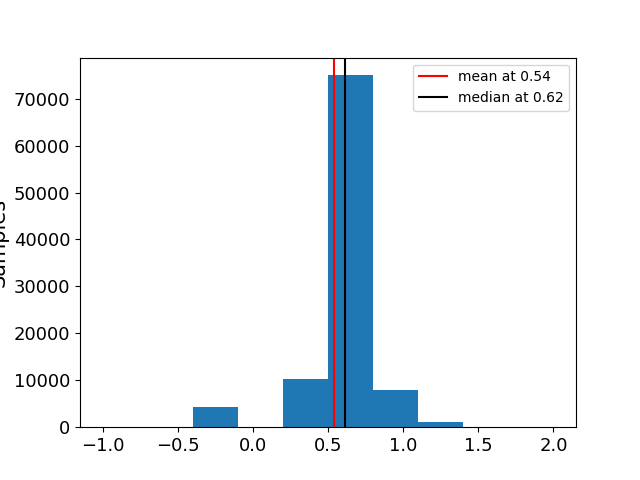
\includegraphics[width=0.995\textwidth]{time-series/autoreg_alphac.png} % first figure itself
        \caption{Alpha}
        \label{fig:aa}
    \end{minipage}\hfill
    \begin{minipage}{0.49\textwidth}
        \centering
        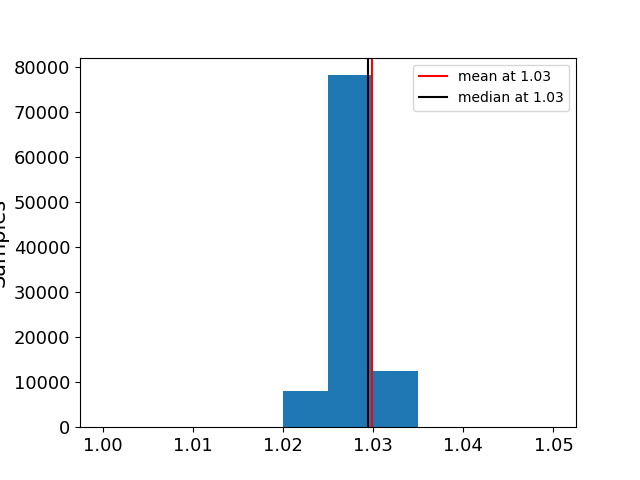
\includegraphics[width=0.995\textwidth]{time-series/autoreg_betac.png} % second figure itself
        \caption{Beta}
        \label{fig:ab}
    \end{minipage}
    
\end{figure}    
        
        % \subsubsection{Moving Average Model}

    \newpage
    \subsection{Data Analysis}
        At times we have some model for the data but we don't know parameters associated with the same. EffPPL is able to get these parameters. 
        
        \subsubsection{Truncated Data}
        When we are given a data from a distribution and it has been truncated but we do not know precisely where it has been truncated we can use this model to find out the possible values at which the data has been truncated. 
        
\begin{listing}[H]\centering
\begin{minted}[linenos, frame=lines,tabsize=2]{ocaml}
let truncated_data obs_points ay () = 
  let* lb = normal (-2.5) 1. in 
  let* ub = normal (2.5) 1. in 
  for i = 0 to (obs_points-1) do 
    observe (mk ay.(i)) 
    (fun x -> 
      if (x < (get lb) || x > (get ub) ) then
        -1000.0
      else 
        (logpdf Primitive.(normal 0. 1.)) x 
    )
  done ;
  lb
\end{minted}
\caption{Truncated data parameter retrieval in EffPPL}


\end{listing}
    
    Here we give priors to \lstinline{lb} and \lstinline{ub}. If a value does not lie within the bounds we give a very large negative number as logpdf(equivalent to 0 probability). Otherwise we use the logpdf of the standard normal distribution(from where we know the truncated data comes). 
    
    We generated data from the standard normal distribution and bounds lying two standard deviations from the mean. Given below are the plots for the estimates of $lb$ and $ub$. As can be seen from figures \ref{fig:lb} and \ref{fig:ub}, they have the highest probability near 2 (or -2) and then it tapers down towards infinity.

\begin{figure}[H]
    \centering
    \begin{minipage}{0.49\textwidth}
        \centering
        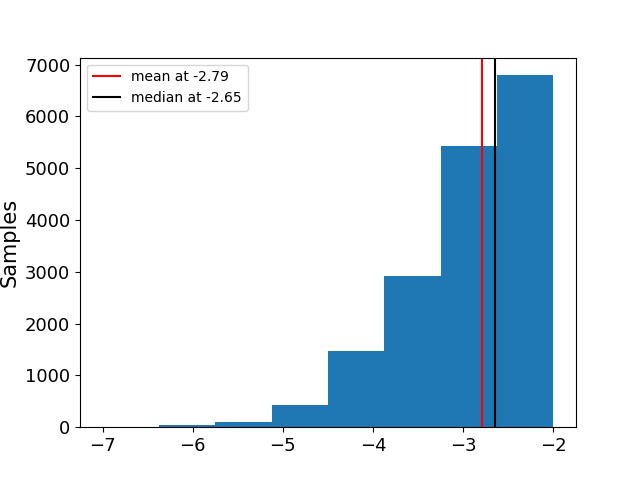
\includegraphics[width=0.99\textwidth]{data/lower_boundc.png} % first figure itself
        \caption{Lower bound Inference}
        \label{fig:lb}
    \end{minipage}
    \begin{minipage}{0.49\textwidth}
        \centering
        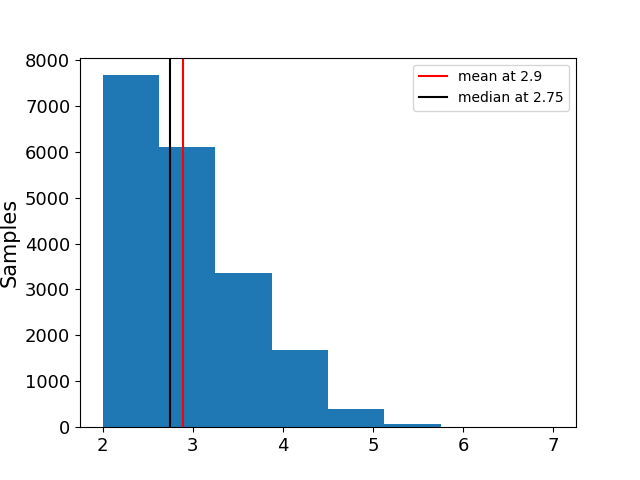
\includegraphics[width=0.99\textwidth]{data/upper_boundc.png} % second figure itself
        \caption{Upper bound inference}
        \label{fig:ub}
    \end{minipage}
    
\end{figure}




        \subsubsection{Missing Data}
        
        Similarly if we do not have the parameters of a particular distribution we can estimate them. Suppose we have a normal distribution whose mean and variance is unknown to us. We can find out these parameters as can be seen below.
\begin{listing}[H]\centering
\begin{minted}[linenos, frame=lines,tabsize=2]{ocaml}
let missing_data obs_points ay () = 
  let* mu = normal ay.(0) 5. in 
  let* si = exp 5.0  in 

  for i = 0 to (obs_points-1) do 
    observe (mk ay.(i)) 
    (fun x -> 
      (logpdf Primitive.(normal (get mu) (get si))) x )
  done ;
  mu
\end{minted}
\caption{Missing parameters}
\end{listing}        
    Here we simply observe the data(\lstinline{ay}) as logpdf of the normal distribution, for parameters \lstinline{mu} and \lstinline{si}.  When given a few points from the standard normal distribution($mu = 0$ and $si = 1$) it was correctly able to predict the \lstinline{mu} and \lstinline{si}. Given below are histograms for the same. As can be seen, \lstinline{mu} has correctly centered around 0 and \lstinline{si} has correctly centered around 1. 
    
    \begin{figure}[H]
    \centering
    \begin{minipage}{0.49\textwidth}
        \centering
        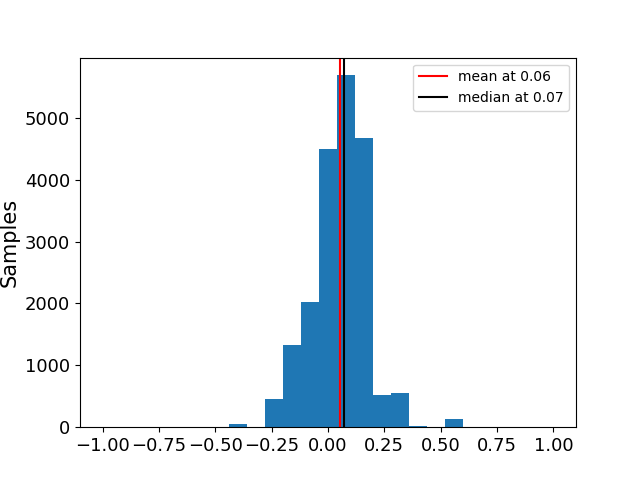
\includegraphics[width=0.99\textwidth]{data/meanc.png} % first figure itself
        \caption{Mean}
        \label{fig:mean_missing_data}
    \end{minipage}
    \begin{minipage}{0.49\textwidth}
        \centering
        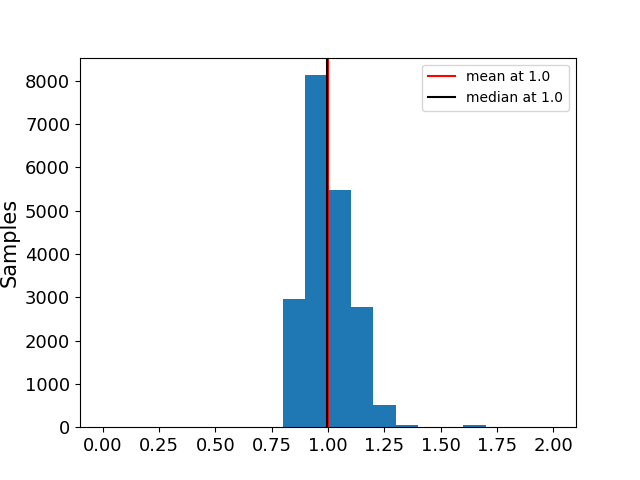
\includegraphics[width=0.99\textwidth]{data/stdevc.png} % second figure itself
        \caption{Std. Dev.}
        \label{fig:std_missing_data}
    \end{minipage}
    
\end{figure}
    The knowledge of these missing parameters can then be used for a various applications such as sampling more data from the same distribution for analysis or for testing against unknown data. 
    \subsection{Sampling}
    \subsubsection{Sum of distributions}
    Figure \ref{norm_sampling} shows an example of sampling from the sum of two normal random variables $ x1 \sim \mathcal{N}(1,3)$ and $x2 \sim \mathcal{N}(1,4)$. Given below is the code for the same.

\begin{listing}[H]\centering
\begin{minted}[linenos, frame=lines,tabsize=2]{ocaml}
let f1 () = 
  let* x1 = normal 1. 3. in
  let* x2 = normal 1. 4. in
  x1 +. x2
\end{minted}

\caption{Sum of normals sampling}
\end{listing}

\begin{figure}[H]
    \centering
    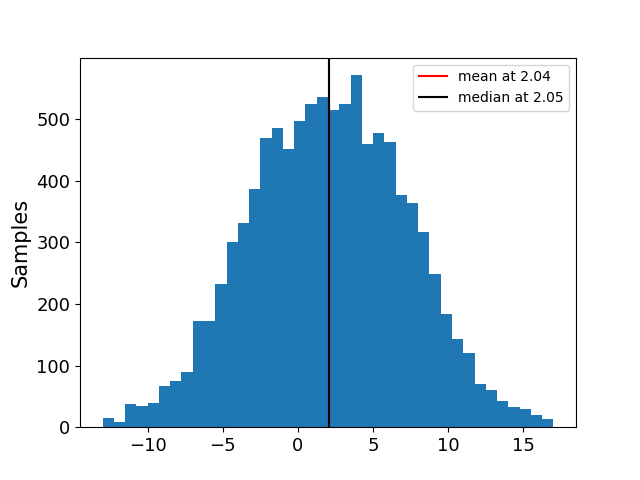
\includegraphics[width=7cm]{sampling/sum_of_normals_samplingc.png}
    \caption{Sum of Normals}
    \label{norm_sampling}
\end{figure}

The output samples have a mean close to 2.0 and a standard deviation close to 5.0, given below is the plot for the same. This is because if $X \sim \mathcal{N}(\mu_1, \sigma_1)$ and $Y \sim \mathcal{N}(\mu_2, \sigma_2)$, then
$X+Y = Z \sim  \mathcal{N}(\mu_1+\mu_2, \sqrt{\sigma^2_1+\sigma^2_2})$


    \subsubsection{Variety of Distributions}\label{vardist}
    
    The EffPPL handles everything via effects, to keep things simple we decided to restrict ourselves to the following distributions
    \begin{enumerate}
        \item Normal Distribution
        \item Gamma Distribution
        \item Beta Distribution
        \item Cauchy Distribution
    \end{enumerate}
    
    However, quite a few distributions such as the Exponential distribution, the Chi-squared distribution and the continuous distribution can be obtained from these primitive distributions. 
    
    We show some samplings from these distributions below:
    
    \begin{figure}[H]
    \centering
    \begin{minipage}{.33\textwidth}
      \centering
      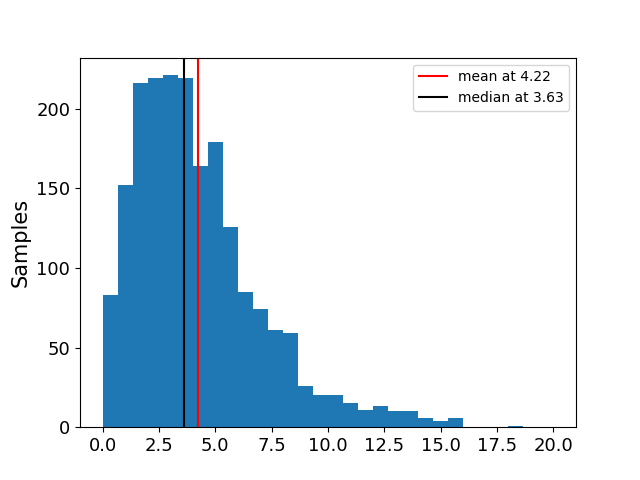
\includegraphics[width=4cm, height=4cm]{sampling/chi2_samplesc.png}
    \end{minipage}%
    \begin{minipage}{.33\textwidth}
      \centering
      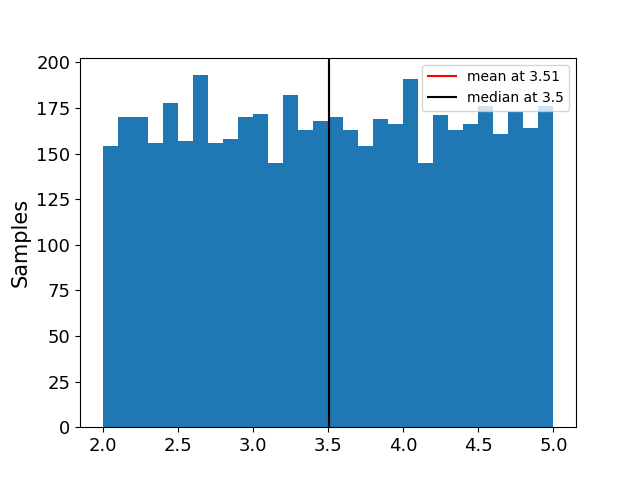
\includegraphics[width=4cm, height=4cm]{sampling/cont_samplesc.png}
    \end{minipage}%
    \begin{minipage}{.33\textwidth}
      \centering
      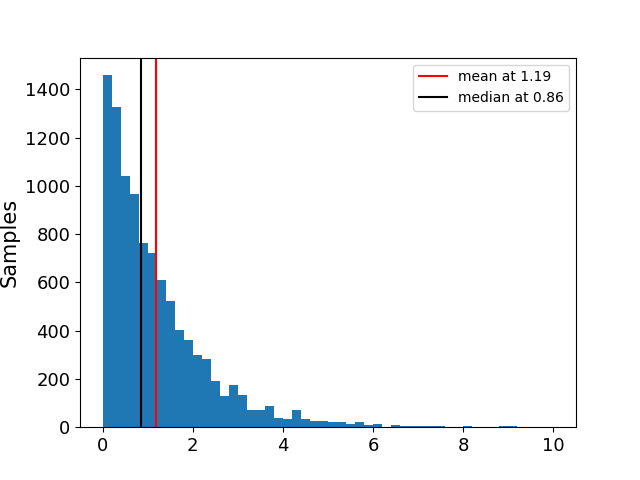
\includegraphics[width=4cm, height=4cm]{sampling/exp_samplesc.png}
    \end{minipage}%
    \par
    \medskip
    \noindent
    \begin{minipage}[t]{.32\textwidth}
      \centering
      \captionof{figure}{$\chi^2(4)$}
    \end{minipage}%
    \begin{minipage}[t]{.32\textwidth}
      \centering
      \captionof{figure}{$Cont(2,5)$}
    \end{minipage}
    \begin{minipage}[t]{.32\textwidth}
      \centering
      \captionof{figure}{$Exp(1)$}
    \end{minipage}%
    \end{figure}
    
    \begin{figure}[H]
    \centering
    \begin{minipage}{.32\textwidth}
      \centering
      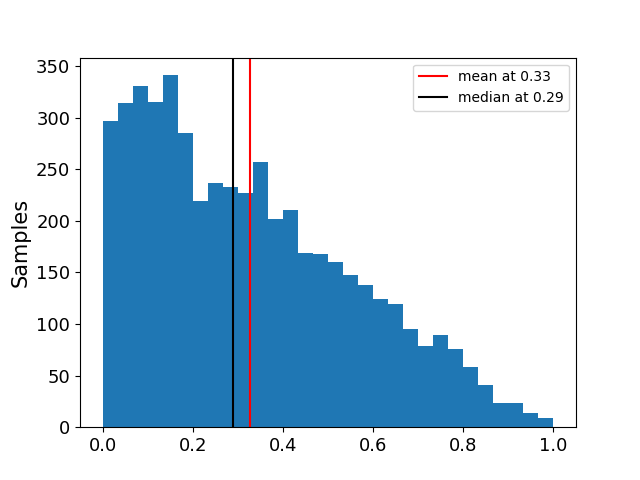
\includegraphics[width=4cm, height=4cm]{sampling/beta_samples_(1,2)c.png}
    \end{minipage}%
    \begin{minipage}{.32\textwidth}
      \centering
      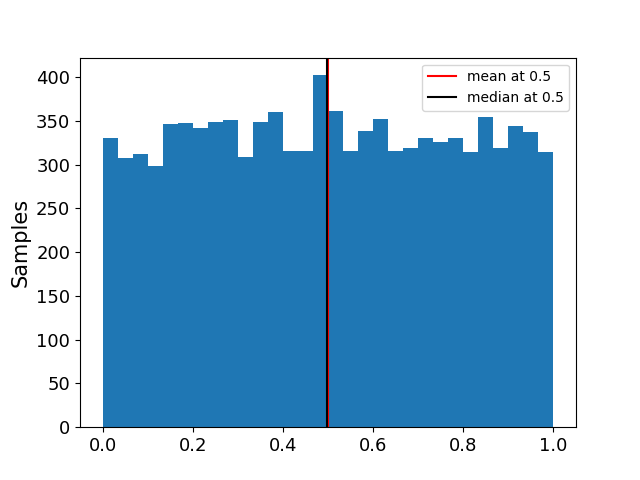
\includegraphics[width=4cm, height=4cm]{sampling/beta_samples_(1,1)c.png}
    \end{minipage}%
    \begin{minipage}{.32\textwidth}
      \centering
      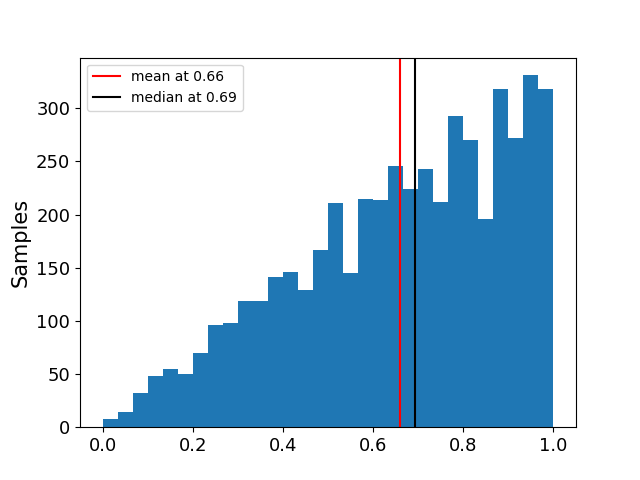
\includegraphics[width=4cm, height=4cm]{sampling/beta_samples_(2,1)c.png}
    \end{minipage}%
    \par
    \medskip
    \noindent
    \begin{minipage}[t]{.32\textwidth}
      \centering
      \captionof{figure}{$\beta(1,2)$}
    \end{minipage}%
    \begin{minipage}[t]{.32\textwidth}
      \centering
      \captionof{figure}{$\beta(1,1)$}
    \end{minipage}
    \begin{minipage}[t]{.32\textwidth}
      \centering
      \captionof{figure}{$\beta(2,1)$}
    \end{minipage}%
    \end{figure}
    
    \subsection{Discrete Models}
    
    While the HMC requires a continuous distribution, as it needs to calculate the gradient of the Probability density function (PDF), we can simulate discreteness by using conditional statements as can be seen in the example below.
    
\begin{listing}[H]\centering
\begin{minted}[linenos, frame=lines,tabsize=2]{ocaml}
let f1 () =
  let* p = uniform 0. 1. in 

  let* flip1 = uniform 0. 1. in 
  let* flip2 = uniform 0. 1. in 
  let* flip3 = uniform 0. 1. in 

  let flip1' = if((get x) > (get flip1)) then 1.0 else 0.0 in 
  let flip2' = if((get x) > (get flip2)) then 1.0 else 0.0 in 
  let flip3' = if((get x) > (get flip3)) then 1.0 else 0.0 in 

  let* total = (mk flip1') +. (mk flip2') +. (mk flip3')  in 
  observe total (fun x-> if x=2.0 then 0.0 else -1000.0);

  total
\end{minted}
\caption{Coin Flips}
\end{listing}

    The above model is used to simulate the following, if we flip 3 coins and observe 2 heads, and we think the prior of the coin weight is uniformly distributed, then what is the posterior? As can be seen, the above example simulates a Bernoulli random variable(\lstinline{flip}' variables) with probability $p$, where $p$ has a prior from the uniform continuous $[0,1]$ distribution. The total is then observed with a function that returns a large negative number to denote its impossible if the total is not 2. For the number of heads equal to 2 and 3 the histogram plots are shown below in figures \ref{fig:2h} and \ref{fig:3h}.
    
    \begin{figure}[H]
    \centering
    \begin{minipage}{0.49\textwidth}
        \centering
        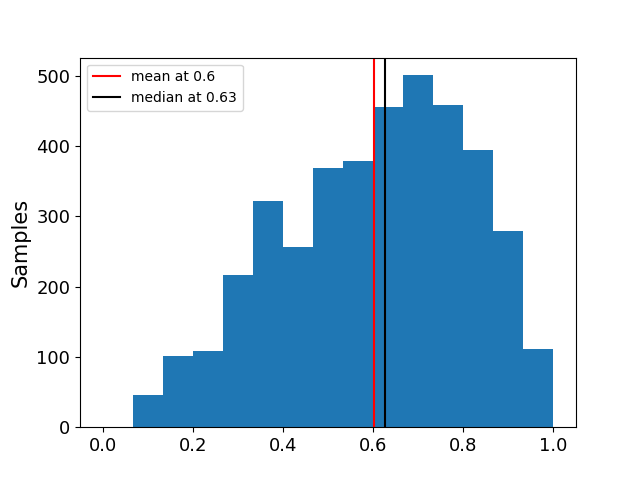
\includegraphics[width=0.995\textwidth]{Coins/coin_weightsc.png} % first figure itself
        \caption{2 heads of 3 flips}
        \label{fig:2h}
    \end{minipage}
    \begin{minipage}{0.49\textwidth}
        \centering
        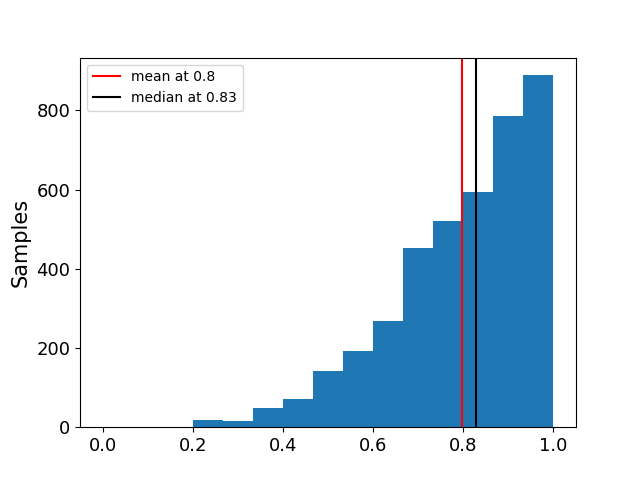
\includegraphics[width=0.995\textwidth]{Coins/coin_weights2c.png}         \caption{3 heads of 3 flips}
        \label{fig:3h}
    \end{minipage}
    
\end{figure}
    
    \newpage
\section{Evaluation}
\label{sec:eval}
    We compare our EffPPL with Stan in this section. Stan has been written in C++ and has witnessed a lot of years of development under many developers. It is considered an industrial strength PPL. Furthermore, it uses the No-U-Turn Sampler, which is widely considered to perform better than the HMC. We are pleasantly surprised that EffPPL compares well with respect to Stan for this example. 
    
    \subsection{Linear Regression}
        
         As a sample example we analyse the performance of two linear regression codes written in Stan and EffPPL against each other inferring the same data. We use the linear regression example mentioned in section \ref{sec:app}. We give both ppls the same data, and see how well they estimate the parameters and in how much time. For Stan, while performing the inference we gave the number of chains as 4 and number of warmup iterations as 7. EffPPL doesn't use chains or warmup iterations as of now so we thought of keeping the value a bit smaller. For larger values of chains/warmup, we would have higher time taken along with better convergence to the mean.
        
        \subsubsection{Parameter Estimation}
            Given below is a plot between the mean slope versus the number of samples drawn for both EffPPL(red) and Stan(blue). We see that while there is a significant difference in the mean slopes in the initial iterations(100 and 316) between Stan and EffPPL, they converge to a value near 3 in the later iterations. 
            \begin{center}
                
            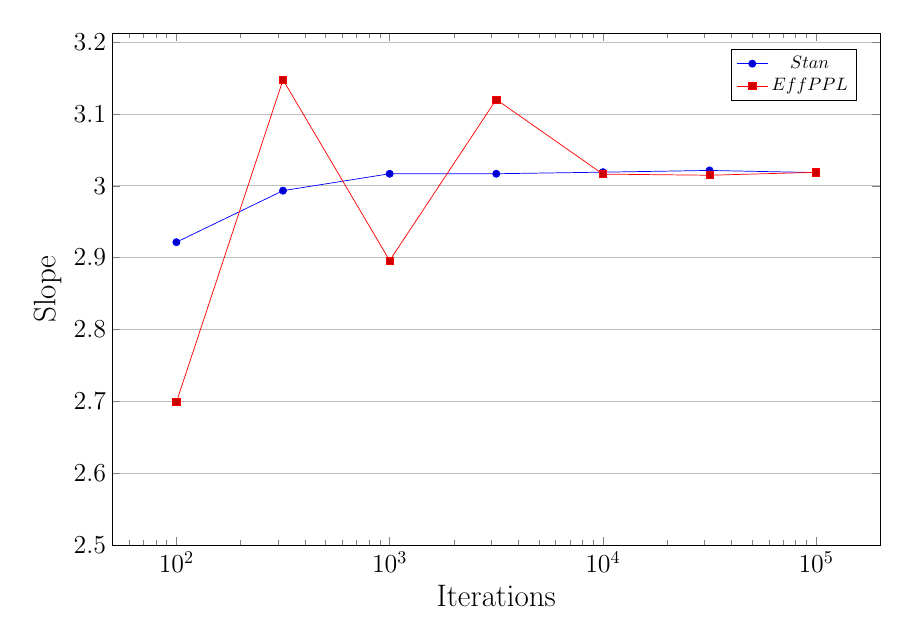
\begin{tikzpicture}[scale=0.65]
    \begin{axis}[
        xmode=log,
    	xlabel={Iterations},
    	ylabel={Slope},
    	label style={font=\LARGE},tick label style={font=\Large},
    % 	x dir=reverse,
    	ytick={2.5, 2.6,2.7, 2.8, 2.9, 3.0, 3.1, 3.2, 3.3},
    	ymajorgrids=true,
    	ymin=2.5,
    	legend pos=north east
    ]
    
    \addplot coordinates {
    	(1e+2,2.92146119)(3.162e+2,2.993174722)(1e+3,3.016667728)(3.162e+3,3.016700522)(1e+4,3.018871833)(3.162e+4,3.021285653)(1e+5,3.018324402)
    };
    \addplot coordinates {
       (1e+2,2.698818)(3.162e+2,3.147426)(1e+3,2.895872)(3.162e+3,3.120045)(1e+4,3.016167)(3.162e+4,3.014606)(1e+5,3.018703)
        };
    % \addplot[color=green, mark=square] coordinates {
    %     (1e-2,35.21)(3.162e-3,54.48)(1e-3,55.94)(0.0005623,55.84)(3.162e-4,58.58)(0.0001778,57.818)(1e-4,59.33)(3.162e-5,57.0)(1e-5,58.78)
    %     };
    
    \legend{$Stan$, $EffPPL$}
    \end{axis}
    \end{tikzpicture}
            \end{center}
            
            Similarly given below is the similar comparative plot between the mean constants obtained by the two libraries. As can be see they both converge to a value close to 1.8 although Stan converges a bit faster.
            
            \begin{center}
            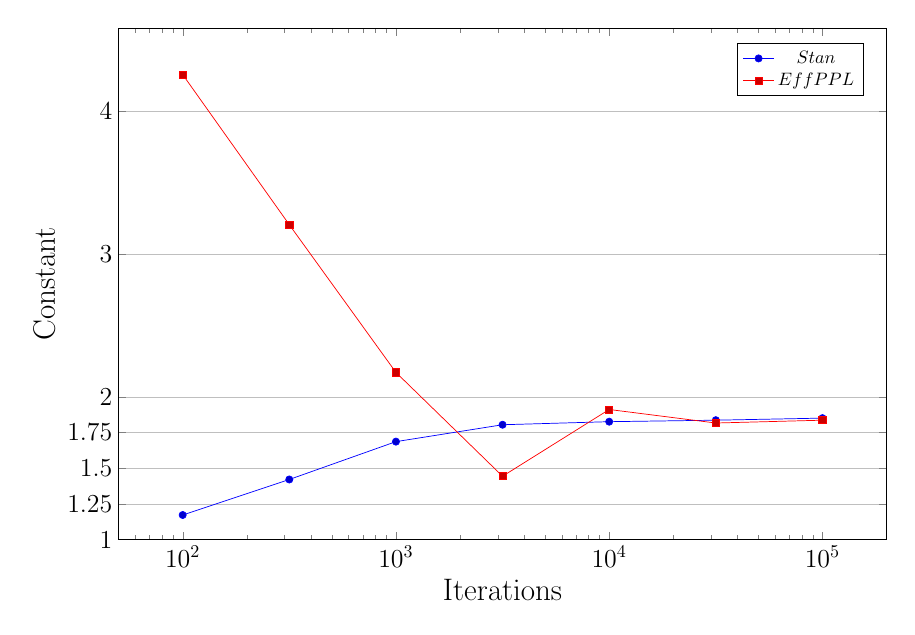
\begin{tikzpicture}[scale=0.65]
            \begin{axis}[
                xmode=log,
            	xlabel={Iterations},
            	ylabel={Constant},label style={font=\LARGE},tick label style={font=\Large},
            	ytick={1.0,1.25,1.5,1.75, 2.0, 3.0, 4.0, 5.0},
            	ymajorgrids=true,
            	ymin=1.0,
            	legend pos=north east
            ]
            
            \addplot coordinates {
            	(100,1.17375251946277)
                (316.227766016838,1.42214970356845)
                (1000,1.68689118307745)
                (3162.27766016838,1.80504911464186)
                (10000,1.82644764253477)
                (31622.7766016838,1.83689824663722)
                (100000,1.85136383471029)
            };
            \addplot coordinates {
               (100,4.254371)
    (316.227766016838,3.20409)
    (1000,2.171045)
    (3162.27766016838,1.444898)
    (10000,1.911708)
    (31622.7766016838,1.817143)
    (100000,1.836922)
                };
            % \addplot[color=green, mark=square] coordinates {
            %     (1e-2,35.21)(3.162e-3,54.48)(1e-3,55.94)(0.0005623,55.84)(3.162e-4,58.58)(0.0001778,57.818)(1e-4,59.33)(3.162e-5,57.0)(1e-5,58.78)
            %     };
            
            \legend{$Stan$, $EffPPL$}
            \end{axis}
            \end{tikzpicture}
                
            \end{center}
            The above graphs show that while Stan is a bit faster at converging. For large enough iterations, we can choose either of the libraries, as both converge to the same values.
            
        \subsubsection{Time Taken}
        Below we also compare the times taken by both with respect to iterations. As can be seen while in the earlier iterations EffPPL takes a lead, Stan is roughly 1.5-2 times faster for large number of iterations in the range of $10^4$-$10^5$. 
         \begin{center}
        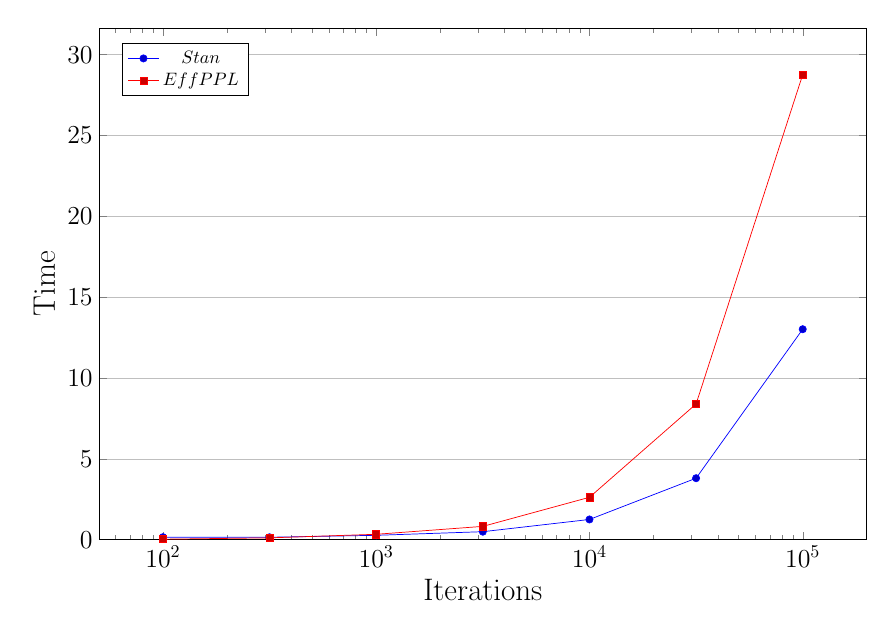
\begin{tikzpicture}[scale=0.65]
        \begin{axis}[
            xmode=log,
        	xlabel={Iterations},
        	ylabel={Time},label style={font=\LARGE},tick label style={font=\Large},
        	ytick={5,0, 10.0, 15.0, 20.0, 25.0, 30.0},
        	ymajorgrids=true,
        	ymin=0,
        	legend pos=north west
        ]
        
        \addplot coordinates {
        	(100,0.16571259498596191)
            (316,0.16009950637817383)
            (1000,0.28029704093933105)
            (3162,0.5036559104919434)
            (10000,1.2594850063323975)
            (31622,3.8108632564544678)
            (100000,13.023686647415161)
        };
        \addplot coordinates {
             (100,0.039566)
            (316.227766016838,0.123267)
            (1000,0.343373)
            (3162.27766016838,0.832276)
            (10000,2.629555)
            (31622.7766016838,8.400285)
            (100000,28.769597)
            };

        \legend{$Stan$, $EffPPL$}
        \end{axis}
        \end{tikzpicture}
            
        \end{center}
        
        While plot seem to be rising exponentially, they are linearly rising. This is because the x-axis is plotted on a logarithmic scale and hence linear plots look exponential. This can be seen from the table \ref{tab:time} denoting the times taken by both libraries below:
        

        \begin{table}[H]\centering
        \begin{tabular}{c|c|c}
        \toprule
        epochs & PyStan (in seconds)   & Effppl(in seconds) \\
        \midrule
        \midrule
        100    & 0.165  & 0.039  \\
        316    & 0.160  & 0.123  \\
        1000   & 0.280  & 0.343  \\
        3162   & 0.503  & 0.832  \\
        10000  & 1.259  & 2.629  \\
        31623  & 3.810  & 8.400 \\
        100000 & \textbf{13.023} & \textbf{28.769} \\
        \bottomrule
        \end{tabular}
        \caption{Times taken}
        \label{tab:time}
        \end{table}
        
        \subsubsection{Dimension}
        
        We also compare how the linear regression in EffPPL performs for larger dimensions. Since we have used a simple list as a data structure we expect it to be $O(p^2)$, where $p$ are the number of parameters. In an optimal setting it will be $O(p)$. 
        
        \begin{center}
        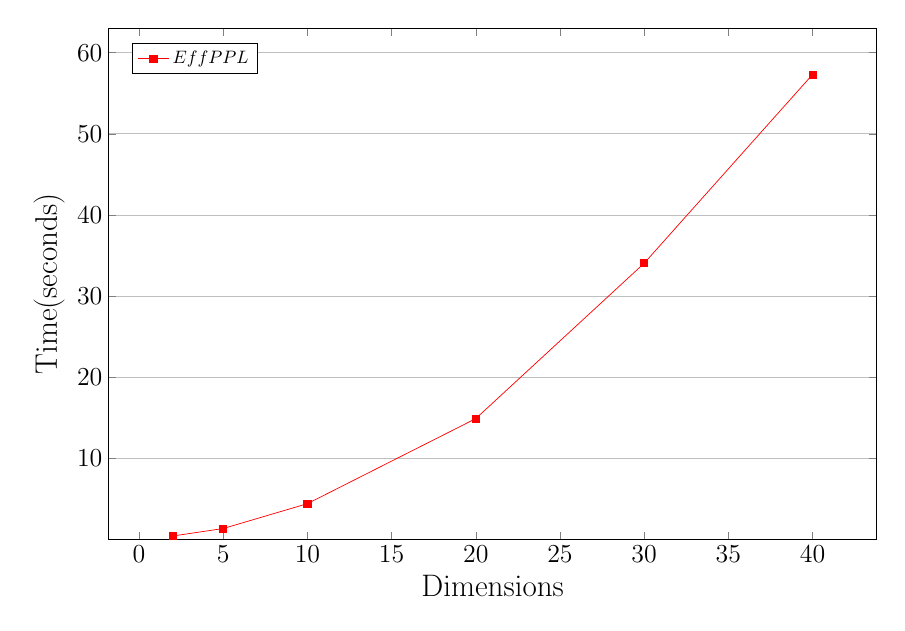
\begin{tikzpicture}[scale=0.65]
        \begin{axis}[
            % xmode=log,
        	xlabel={Dimensions},
        	ylabel={Time(seconds)},label style={font=\LARGE},tick label style={font=\Large},
        	ytick={10.0, 20.0, 30.0, 40.0, 50.0, 60.0},
        	ymajorgrids=true,
        	ymin=0,
        	legend pos=north west
        ]
        
        \addplot[color = red, mark=square*] coordinates {
        	(2.0, 0.473)
        	(5.0, 1.394)
        	(10.0,4.457)
        	(20.0,14.935)
        	(30.0,34.064)
        	(40.0,57.304)
        };
        
        \legend{$EffPPL$}
        \end{axis}
        \end{tikzpicture}
        \end{center}
        
        As can be seen the plot has a greater than linear component associated with it. However, even for a 40-dimensional linear regression it was able to go through a 1000 iterations with 100 points within a minute.
        

\section{Further Work}

While the inference algorithm is performing well, there are some places where the library can be improved. These are:
\begin{enumerate}
    \item Using a No-U-Turn Sampler instead of the Hamiltonian Monte Carlo. This would save users from choosing appropriate step sizes and iterations.
    \item Adding an inference algorithm that can also deal with discrete models. Currently we have to use conditionals on the continuous distributions to get discrete models. 
    \item Using alternative data-structures to improve the efficiency of the PPL for higher dimensions
    \item Adding a Multicore effect scheduler to make the library parallelised. 
\end{enumerate}

\section{Appendix}

Given below is a table of keywords that are used in the EffPPL library
\begin{table}[H]
	
    \caption{EffPPL keywords and primitives}
	\begin{tabular}{|c|c|c|}
		\toprule
		Keyword & Function type & Use \\	
		\midrule
		\midrule
		\texttt{let*}        &   {\small \texttt{t -> (t -> t ) ->  t }} &  
		A primitive for declaring variables \\ \midrule
		\texttt{normal}        & {\small \texttt{ float -> float -> t }}&  
		\bigcell{c}{Given mean and std. dev. samples \\numbers from the normal/gaussian distribution} \\ \midrule
		\texttt{cauchy}        & {\small \texttt{ float -> float -> t }}&  
		\bigcell{c}{Given loc and scale \\samples numbers from the cauchy distribution } \\ \midrule
		\texttt{beta}        &  {\small \texttt{float -> float -> t}} &   
		\bigcell{c}{Given a and b \\samples numbers from the beta distribution } \\ \midrule
		\texttt{gamma}        & {\small \texttt{float -> float -> t }} &   
		\bigcell{c}{Given shape and scale \\samples numbers from the gamma distribution } \\ \midrule
		\texttt{exp}        &  {\small \texttt{float -> t }}&   
		\bigcell{c}{Given rate samples numbers\\ from the exponential distribution } \\ \midrule
		\texttt{chi2}        & {\small \texttt{ float -> t}} &    
		\bigcell{c}{Given degrees of freedom\\ samples numbers from the exponential distribution } \\ \midrule
		\texttt{uniform}        & {\small \texttt{ float -> float -> t }}&    
		\bigcell{c}{Given start and end\\ samples numbers from the uniform distribution } \\ \midrule
		\texttt{hmc}        & \bigcell{c}{{\small \texttt{( unit ->  t)  -> int ->}} \\{\small \texttt{float -> int -> float list list}}}   &  
		\bigcell{c}{Given function, leapfrog iterations, step size\\ and number of epochs returns a list of samples\\ having length number of epochs }\\ \midrule
		\texttt{observe}        & {\small \texttt{ t -> (float -> float) -> unit}}  &   
		\bigcell{c}{Given a variable to observe and function that \\returns the logpdf it takes this observation \\ into account while doing inference}\\
		\bottomrule
	\end{tabular}
	\label{key}
\end{table}
\newpage



\bibliographystyle{unsrt}
\bibliography{mybib}
\end{document}